\documentclass[a4paper,twoside,twocolumn]{article}
\usepackage{blindtext}  
\usepackage{geometry}

% Chinese support
\usepackage[UTF8, scheme = plain]{ctex}

% Page margin layout
\geometry{left=2.3cm,right=2cm,top=2.5cm,bottom=2.0cm}

\usepackage{etoolbox}
\patchcmd{\thebibliography}{\section*{\refname}}{}{}{}

\usepackage{cuted}

\usepackage{listings}
\usepackage{xcolor}
\usepackage{geometry}
\usepackage{amsmath}
\usepackage{float}
\usepackage{hyperref}

\usepackage{graphics}
\usepackage{graphicx}
\usepackage{subfig}
\usepackage{subfloat}
\usepackage{epsfig}
\usepackage{stfloats}
\usepackage{float}

\usepackage{algorithm}
\usepackage[noend]{algpseudocode}

\usepackage{booktabs}
\usepackage{threeparttable}
\usepackage{longtable}
\usepackage{listings}
\usepackage{tikz}
\usepackage{multicol}

% cite package, to clean up citations in the main text. Do not remove.
\usepackage{cite}

\usepackage{color,xcolor}

%% The amssymb package provides various useful mathematical symbols
\usepackage{amssymb}
%% The amsthm package provides extended theorem environments
\usepackage{amsthm}
\usepackage{amsfonts}
\usepackage{enumerate}
\usepackage{enumitem}
\usepackage{listings}
\usepackage{makecell}

\usepackage{indentfirst}
\setlength{\parindent}{2em} % Make two letter space in the first paragraph
\usepackage{setspace}
\linespread{1.5} % Line spacing setting
\usepackage{siunitx}
\setlength{\parskip}{0.5em} % Paragraph spacing setting

% \usepackage[contents =22920202204622, scale = 10, color = black, angle = 50, opacity = .10]{background}

\renewcommand{\figurename}{图}
\renewcommand{\lstlistingname}{代码} 
\renewcommand{\tablename}{表格}
\renewcommand{\contentsname}{目录}
\floatname{algorithm}{算法}

\graphicspath{ {images/} }

%%%%%%%%%%%%%
\newcommand{\StudentNumber}{22920202204622 \ 2292020220786 \ 22920202204623 \ 22920202202780}  % Fill your student number here
\newcommand{\StudentName}{熊恪峥 \ 杨夏婕 \ 徐杰 \ 黄彬茹}  % Replace your name here
\newcommand{\PaperTitle}{CPPBP: 高扩展性的神经网络框架}  % Change your paper title here
\newcommand{\PaperType}{面向对象的程序设计(C++)} % Replace the type of your report here
\newcommand{\Date}{2022年6月1日}
\newcommand{\College}{信息学院}
\newcommand{\CourseName}{算法设计与分析}
%%%%%%%%%%%%%

%% Page header and footer setting
\usepackage{fancyhdr}
\usepackage{lastpage}
\pagestyle{fancy}
\fancyhf{}
% This requires the document to be twoside
\fancyhead[LO]{\texttt{\PaperTitle }}
\fancyhead[LE]{\texttt{\PaperType}}
\fancyhead[R]{\texttt{第{\thepage}页,共\pageref*{LastPage}页}}


\title{\PaperTitle}
\author{\StudentName}
\date{\Date}

\lstset{
	basicstyle          =   \sffamily,          % 基本代码风格
	keywordstyle        =   \bfseries,          % 关键字风格
	commentstyle        =   \rmfamily\itshape,  % 注释的风格,斜体
	stringstyle         =   \ttfamily,  % 字符串风格
	flexiblecolumns,   
	showspaces          =   false,  % 是否显示空格,显示了有点乱,所以不现实了
	numberstyle         =   \zihao{-5}\ttfamily,    % 行号的样式,小五号,tt等宽字体
	showstringspaces    =   false,
	captionpos          =   t,      % 这段代码的名字所呈现的位置,t指的是top上面
	frame               =   lrtb,   % 显示边框
	numbers             =   none	   % 不显示行号
}

\lstdefinestyle{PythonStyle}{
	language        =   Python, % 语言选Python
	basicstyle      =   \zihao{-5}\ttfamily,
	numberstyle     =   \zihao{-5}\ttfamily,
	keywordstyle    =   \color{blue},
	keywordstyle    =   [2] \color{teal},
	stringstyle     =   \color{magenta},
	commentstyle    =   \color{red}\ttfamily,
	breaklines      =   true,   % 自动换行,建议不要写太长的行
	columns         =   fixed,  % 如果不加这一句,字间距就不固定,很丑,必须加
	basewidth       =   0.5em,
}

\lstdefinestyle{CppStyle}{
	language        =   c++,
	basicstyle      =   \zihao{-5}\ttfamily,
	numberstyle     =   \zihao{-5}\ttfamily,
	keywordstyle    =   \color{blue},
	keywordstyle    =   [2] \color{teal},
	stringstyle     =   \color{magenta},
	commentstyle    =   \color{red}\ttfamily,
	breaklines      =   true,   % 自动换行,建议不要写太长的行
	columns         =   fixed,  % 如果不加这一句,字间距就不固定,很丑,必须加
	basewidth       =   0.5em,
}

\algnewcommand\algorithmicinput{\textbf{Input:}}
\algnewcommand\algorithmicoutput{\textbf{Output:}}
\algnewcommand\Input{\item[\algorithmicinput]}%
\algnewcommand\Output{\item[\algorithmicoutput]}%

\usetikzlibrary{positioning, shapes.geometric}

\setcounter{tocdepth}{2}

\begin{document}
	
%%%%%%%%%%%%%%%%%%%%%%%%%%%%%%%%%%%%%%%%%%%%
\makeatletter % change default title style
\renewcommand*\maketitle{%
	\begin{center} 
		\bfseries  % title 
		{\LARGE \@title \par}  % LARGE typesetting
		\vskip 1em  %  margin 1em
		{\global\let\author\@empty}  % no author information
		{\global\let\date\@empty}  % no date
		\thispagestyle{empty}   %  empty page style
	\end{center}%
	\setcounter{footnote}{0}%
}
\makeatother
%%%%%%%%%%%%%%%%%%%%%%%%%%%%%%%%%%%%%%%%%%%%

\onecolumn
	
\thispagestyle{empty}

\vspace*{1cm}

\begin{figure}[h]
	\centering
	
\includegraphics[width=4.0cm]{logo.png}
\end{figure}

\vspace*{1cm}

\begin{center}
	\Huge{\textbf{\PaperType}}
	
	\Large{\PaperTitle}
\end{center}

\vspace*{1cm}

\begin{table}[h]
	\centering	
	\begin{Large}
		\renewcommand{\arraystretch}{1.5}
		\begin{tabular}{p{3cm} p{5cm}<{\centering}}
			姓\qquad 名 & \StudentName  \\
			\hline
			学\qquad号 & \StudentNumber \\
			\hline
			日\qquad期 & \Date  \\
			\hline
			学\qquad院 & \College  \\
			\hline
			课程名称 & \CourseName  \\
			\hline
		\end{tabular}
	\end{Large}
\end{table}

\newpage

\title{
	\Large{\textcolor{black}{\PaperTitle}}
}

\maketitle

	
\tableofcontents
 
\newpage
\setcounter{page}{1}

\twocolumn

\begin{strip}
	\centering
	\LARGE \PaperTitle
	\vspace*{0.5cm}
	\normalsize
	\begin{minipage}{\linewidth}
		\centering
		\begin{minipage}[t]{1.2in}
			\centering
			熊恪峥 \\
			22920202204622 \\
		\end{minipage}
		\begin{minipage}[t]{1.2in}
			\centering
			杨夏婕 \\
			2292020220786
		\end{minipage}
		\begin{minipage}[t]{1.2in}
			\centering
			徐杰 \\
			22920202204623
		\end{minipage}\begin{minipage}[t]{1.2in}
			\centering
			黄彬茹 \\
			22920202202780
		\end{minipage}
	\end{minipage}
	\vspace*{0.25cm}
\end{strip}

\begin{spacing}{1.2}

\noindent\textbf{摘要 }
反向传播算法在深度学习领域有着重要的地位。它是训练一个神经网络的理论基础。由
全连接层组成的MLP是一种基本的神经网络结构。同时,近两年来\cite{mlpmixer}、\cite{resmlp}
证实了纯MLP组成的网络结构,在计算机视觉领域并不是完全低效的,可以在分类任务上
达到卷积神经网络级别的性能。并且更少的归纳偏置带来了更强大的拟合能力和泛化能力。
本项目实现了一个静态建图的、高可扩展性的基于反向传播算法的神经网络框架\emph{cppbp},
提供了统一的接口以保证代码的简洁可读,以及常用的优化器、损失函数、正则化方法的实现。
代码已经在\url{https://github.com/SmartPolarBear/cppbp}上开源。

\vspace*{0.15cm}

\section{架构设计}

架构设计是提高可扩展性的重要保障。我们首先对该框架的需求进行了合理划分,如
图~\ref{fig:mdl_spl}。我们将整体工作流划分为模型构建、数据处理、训练与测试、
可持久化与部署四个部分。
\begin{figure}[htb]
	\centering
	\caption{模块划分}
	\label{fig:mdl_spl}
	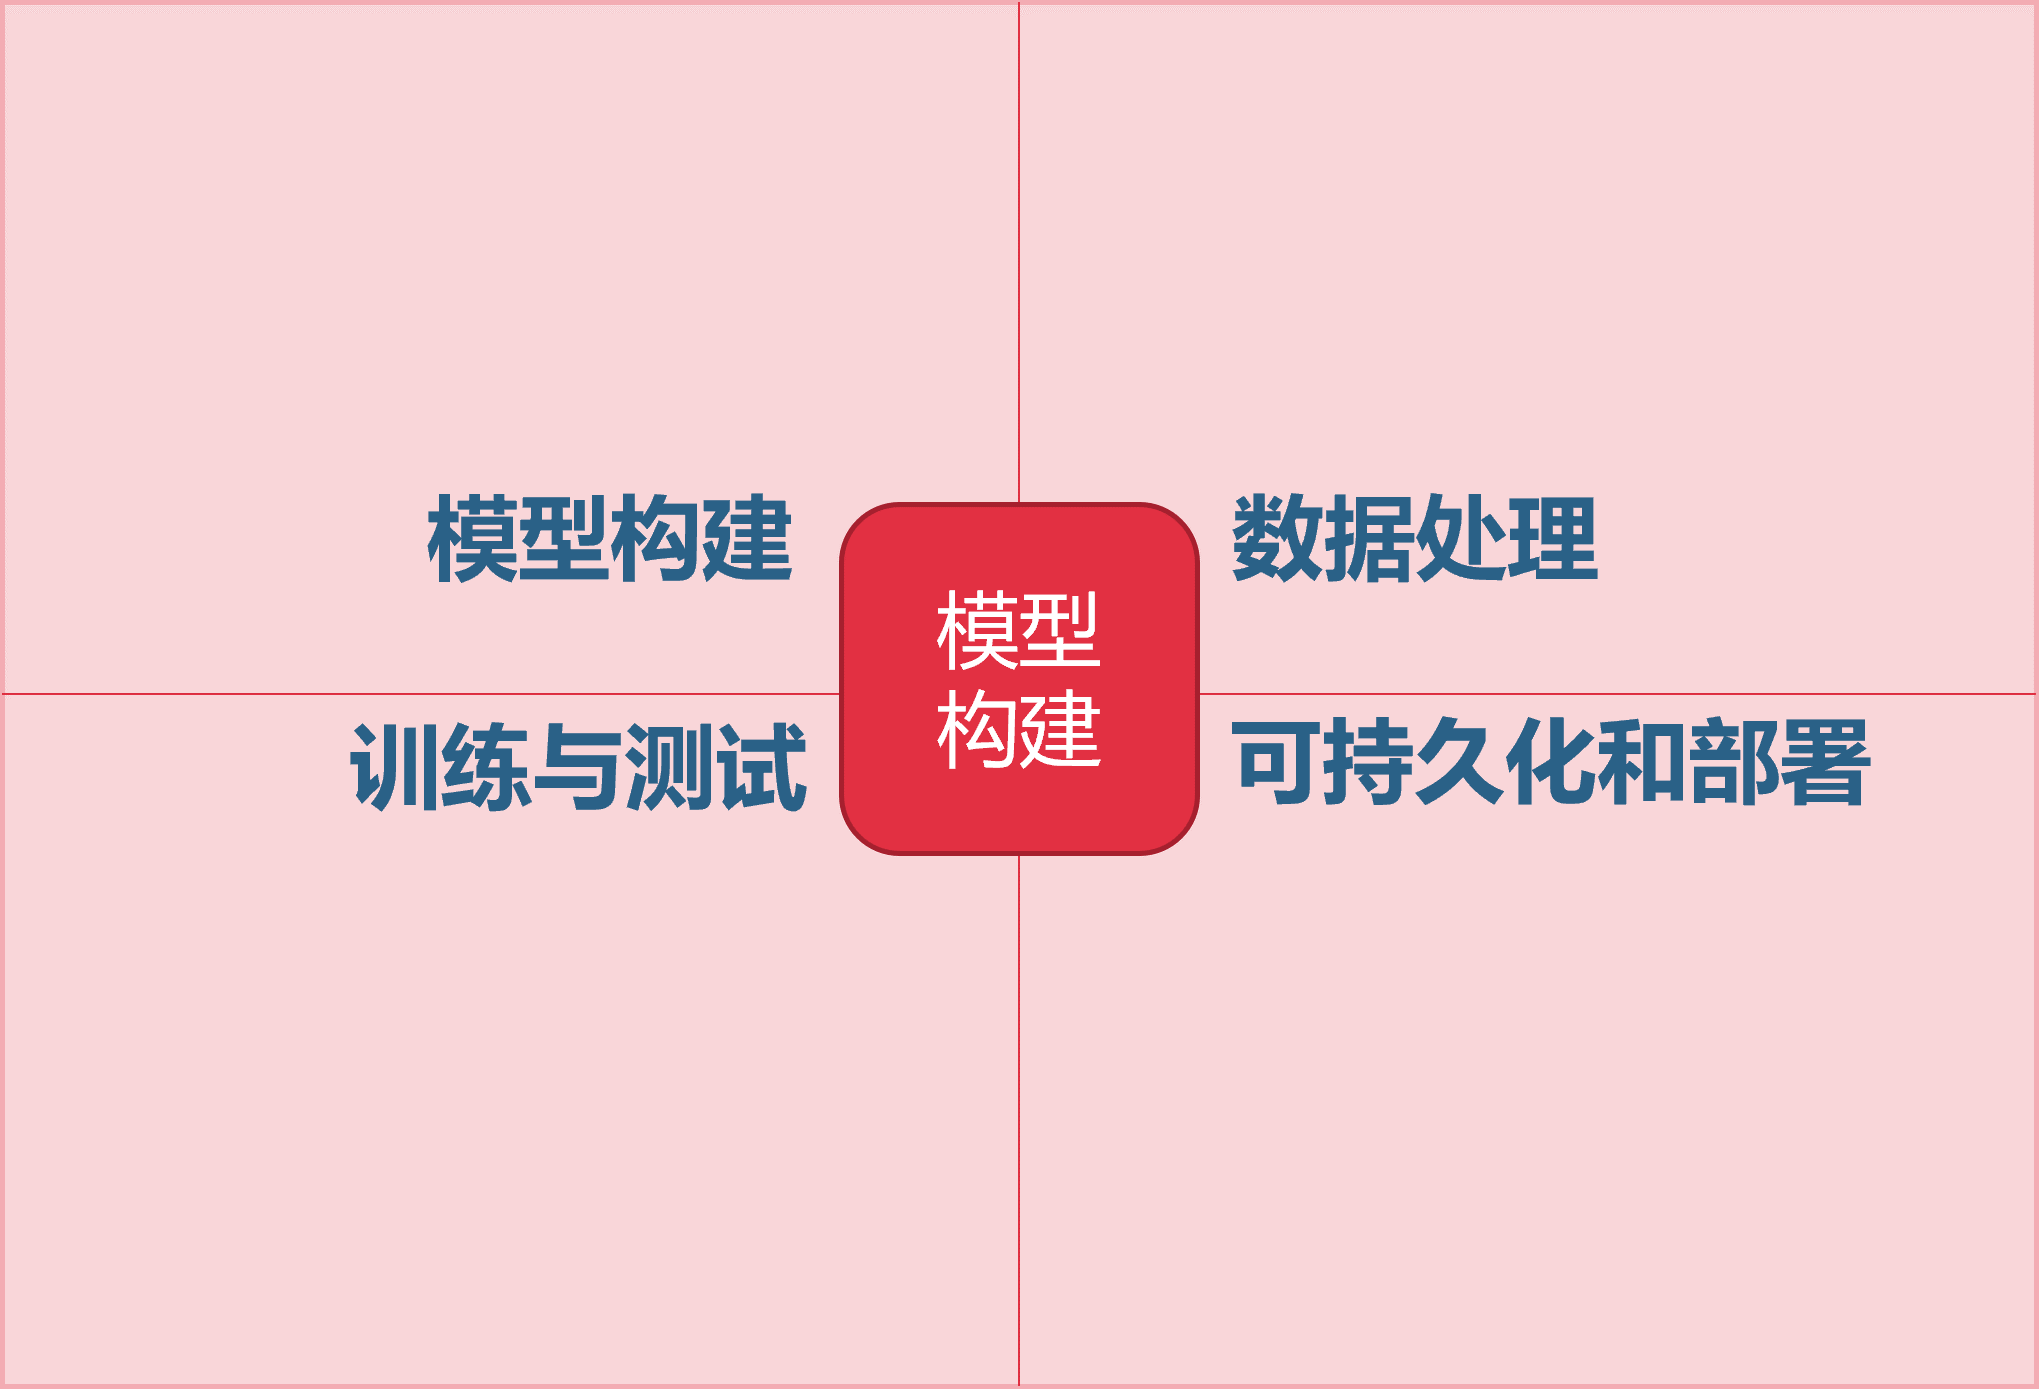
\includegraphics[width=0.35\textwidth]{module_split.png}
\end{figure}

这四个部分分别完成模型的搭建与反向传播的处理;数据的读入、打乱、增强;训练流程搭建
和训练效果测试;模型参数的保存读取功能。

\subsection{高可扩展性与整体设计}

从可扩展性的视角考虑,我们首先就上述任务的中最普遍、最一般的需求设计了一组接口。C++没有
语言级别的接口定义,像Java和C\#等语言具备的那样。因此我们严格限制被称为\emph{接口}的类
的内容,使其仅仅包含纯虚函数以供子类重写。

然后,我们从构建神经网络的任务中最常见的需求出发,实现具体的类来完成模块的整体功能。包括
优化器、全连接层、DropOut层和LayerNorm层、数据加载器等内容,具体内容如图~\ref{fig:comps}。

\begin{figure*}[htb]
	\centering
	\caption{主要功能}
	\label{fig:comps}
	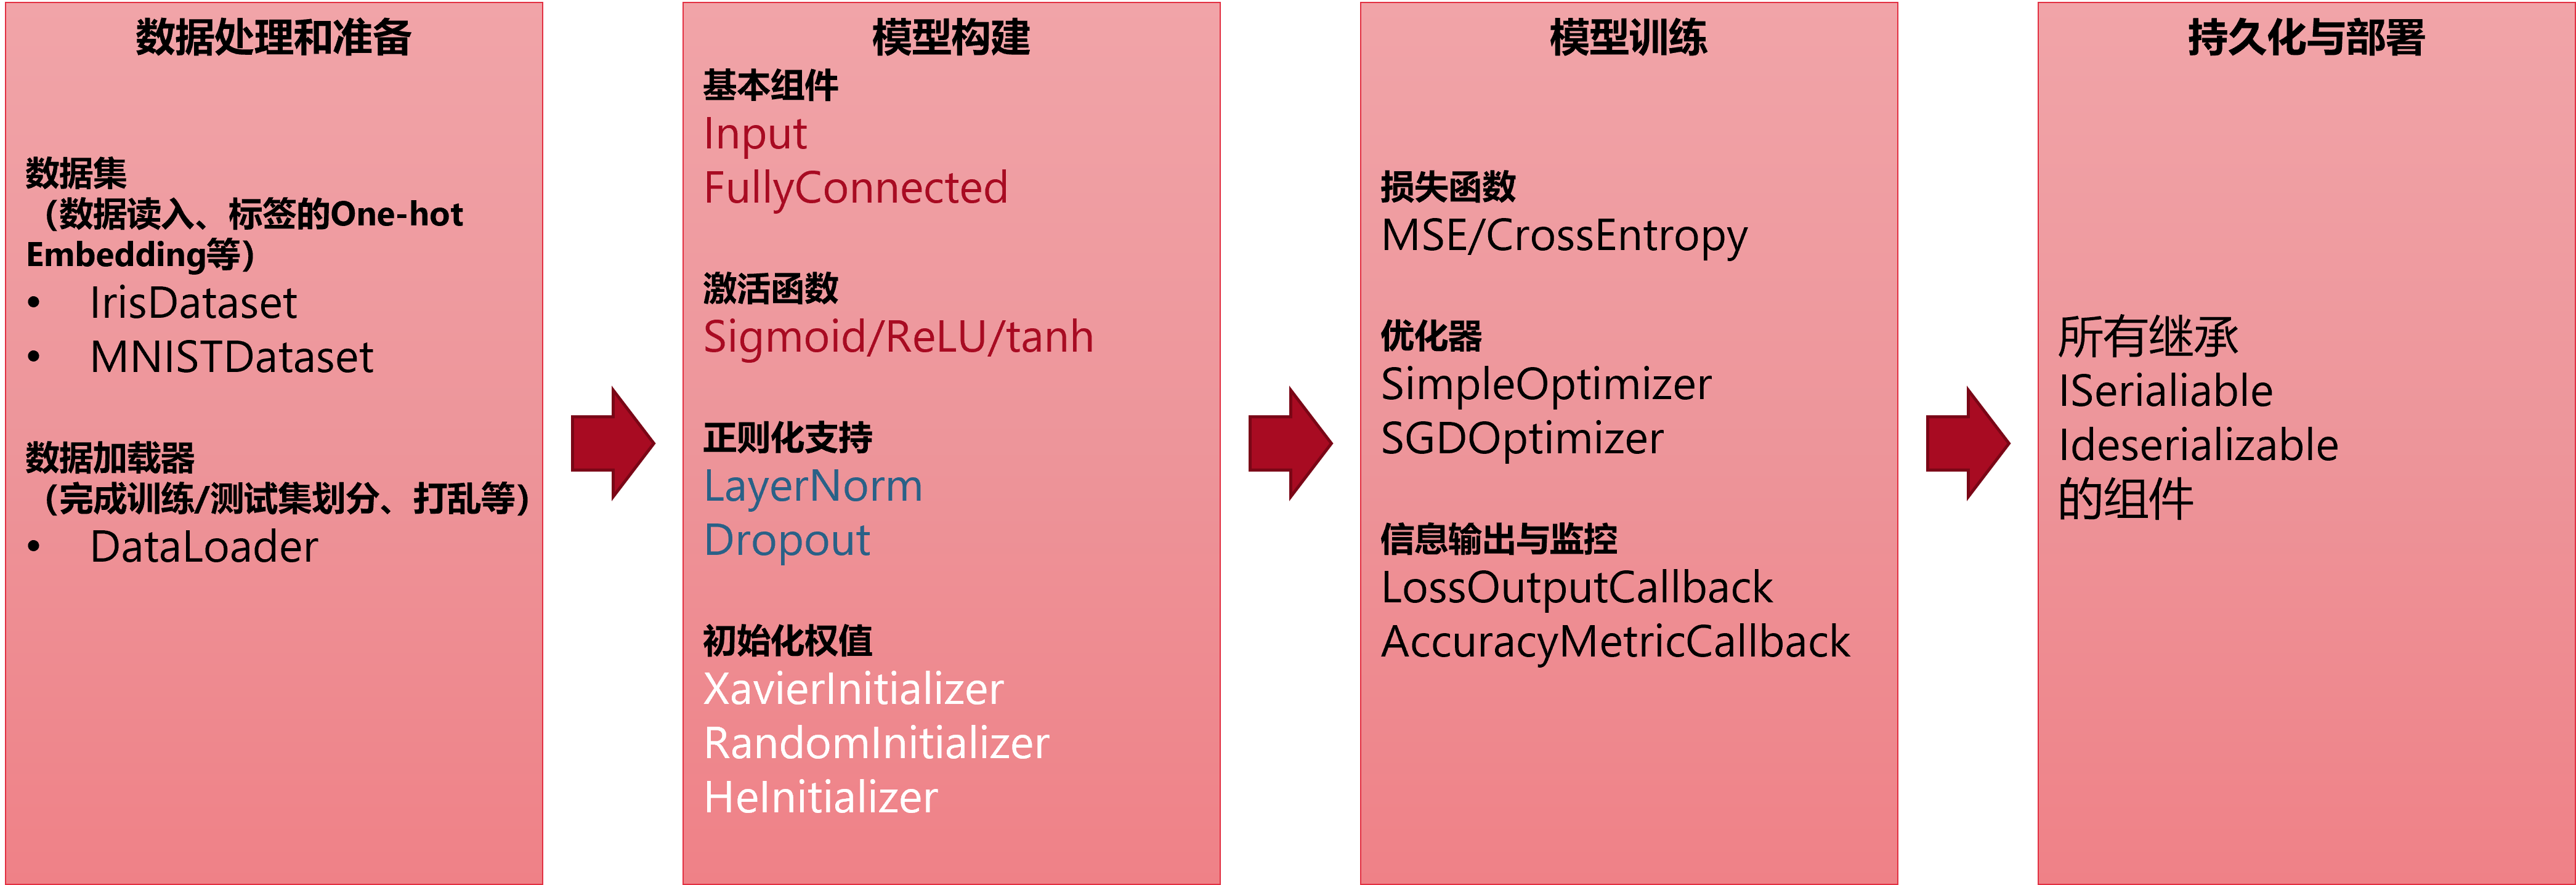
\includegraphics[width=0.8\textwidth]{comps.png}
\end{figure*}

通过这种实现方法,我们既保证了内置组件的接口风格统一,也保证了任何自定义组件只要实现
对应的接口,就可以和其他内置组件无缝协同工作,良好地实现了高可扩展性愿景。


\subsection{高可用性与API设计}

在API设计上,为了保证良好的代码可读性,我们坚持让代码的形式结构和执行逻辑相统一
的设计理念。即\emph{代码的文本本身应当对运行时发生的事有一种恰当的隐喻}。在此基础上,
我们积极保证接口设计和现代C++的STL库设计相适应的原则。

这里以管道运算符的设计为例。我们实现了管道运算符(Pipe Operators)以表达层之间的连接。
该运算符的使用如代码~\ref{code:pipe}中所示。

\begin{lstlisting}[language=c++,style=CppStyle,caption={管道运算符},label={code:pipe}]
Input in{4};
FullyConnected fc1{5, relu};
FullyConnected fc2{8, sigmoid};
DropOut drop1{0.05};
FullyConnected fc3{12, sigmoid};
FullyConnected out{3, softmax};
CrossEntropyLoss loss{};
Model model{in | fc1 | fc2 | drop1 | fc3 | out, loss};
\end{lstlisting}

其中最后一行使用管道运算符连接各层,在此过程中计算图的构建和各层参数的调整会自动完成。这样使得构建模型
的过程看起来更加简单直接。这种设计来自于C++20 Ranges\footnote{Ranges library \url{https://en.cppreference.com/w/cpp/ranges}}
对范围适配器进行复合时使用的设计。

正如Bjarne Stroustrup的论文\textit{Thriving in a Crowded and Changing World: C++ 2006-2020}中的观点\cite{stroustrup2020thriving},
Ranges是对C++ STL的重要改进。我们借鉴其设计,能够面向未来地使我们的库与未来的C++标准库更为接近,使得初学者
容易学习、容易上手、容易理解。

\section{实现与功能}

\subsection{反向传播公式的改进实现}

为了更好地实现高可扩展性的架构设计,我们需要改进常见的的反向传播公式。
\begin{equation}
	\label{eqn:bpnaive}
	\begin{aligned}
		\frac{\partial L}{\partial \mathbf{W}}&=L^{'}(\mathbf{z^{(L)}})\cdot f^{'}(\mathbf{z^{(L)}})\cdot \mathbf{a^{(L-1)}}\\
		\sigma^{(L)}&=L^{'}(\mathbf{z^L})\cdot f^{'}(\mathbf{z^L})
	\end{aligned}
\end{equation}
反向传播公式计算损失函数对最后一层参数的梯度的公式的的常见形式如\eqref{eqn:bpnaive}。
这种写法有较强的局限性。例如不是所有的激活函数$f$都是一元函数。一个常用的多元激活函数是Softmax函数,
它的定义是$f(x_j;\mathbf{x})=\frac{e^{x_j}}{\sum_{x_i\in \mathbf{x}} e^{x_i}}$,对于这种多元函数,该公式是无法处理的。
因此我们从最根本的链式法则出发使得反向传播公式更加符合我们的高可扩展性愿景。设最后一层激活值为$\mathbf{z}$,有\eqref{eqn:bp_derive1}
\begin{equation}
	\label{eqn:bp_derive1}
	\begin{aligned}
		\frac{\partial L}{\partial \mathbf{x}}=
		\frac{\partial L}{\partial \mathbf{z}}\cdot\frac{\partial \mathbf{z}}{\partial \mathbf{x}}
	\end{aligned}
\end{equation}
则各个分量有\eqref{eqn:bp_derive2}
\begin{equation}
	\label{eqn:bp_derive2}
	\begin{aligned}
		\frac{\partial L}{\partial x_i}=
		\sum_j\frac{\partial L}{\partial z_j}\cdot\frac{\partial z_j}{\partial \mathbf{x_i}}
	\end{aligned}
\end{equation}
设最后一层各神经元有激活函数$f_1, f_2, \ldots, f_n$,令
\(
J=\begin{bmatrix}
	\frac{\partial f_1}{\partial x_1}&\cdots&\frac{\partial f_1}{\partial x_n}\\
	\vdots&\vdots&\vdots\\
	\frac{\partial f_n}{\partial x_1}&\cdots&\frac{\partial f_n}{\partial x_n}\\
\end{bmatrix}
\),
\(
d^\mathsf{T}=\begin{bmatrix}
	\frac{\partial L}{\partial x_1}&\cdots&\frac{\partial L}{\partial x_n}\\
\end{bmatrix}
\)
则\eqref{eqn:bp_derive1}可以写成\eqref{eqn:bp_derive3}
\begin{equation}
	\label{eqn:bp_derive3}
	\begin{aligned}
		\frac{\partial L}{\partial \mathbf{x}}=
		d^\mathsf{T} J
	\end{aligned}
\end{equation}

这样做的好处不仅仅是能够处理Softmax这样的多元激活函数,更重要的是矩阵-向量的乘法可以良好地
利用SIMD(Single Instruction Multiple Data)指令进行并行化处理,能够充分利用现代
硬件的性能。

\subsection{激活函数}
激活函数是重要的组件。非线性的激活函数是多层神经网络能够拟合任意复杂的函数的强大能力的重要基础。
我们主要实现了四种激活函数:ReLU、Softmax、Tanh、Sigmoid。

每个激活函数都要实现$IActivationFunction$中的$eval$和$derive$,分别进行求值和求导,求导的对象包括标量和向量。如代码~\ref{code:actfun}

\begin{lstlisting}[language=c++,style=CppStyle,caption={接口$IActivationFunction$},label={code:actfun}]
class IActivationFunction
        : public base::ITypeId
{
public:
    virtual double operator()(double x) = 0;

    virtual double eval(double x) = 0;

    virtual double derive(double y) = 0;

    virtual Eigen::VectorXd eval(Eigen::VectorXd x) = 0;

    virtual Eigen::MatrixXd derive(Eigen::VectorXd y) = 0;

    virtual std::shared_ptr<IWeightInitializer> default_initializer() = 0;
};
\end{lstlisting}

\subsubsection{$ReLU$函数}

ReLU(Rectified Linear Unit)是一个分段线性函数,如果输入为正,直接输出;否则,输出为零。函数图像如下:

\begin{figure}[htb]
	\centering
	\caption{ReLU}
	\label{fig:relu}
	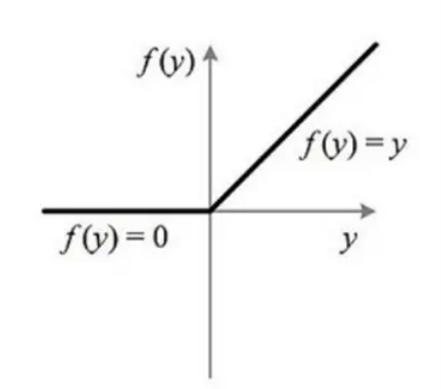
\includegraphics[width=0.4\textwidth]{relu.png}
\end{figure}


公式是
$
f(x)=\max(0,x)
$

ReLU函数的求导结果也较为简单,在$x>0$处为1,否则为0。ReLU的导数恒为1,不容易
导致梯度消失的问题,在深度神经网络模型中非常常用。

\subsubsection{$Sigmoid$函数}

Sigmoid函数也是常被用作神经网络的激活函数,它将输入映射到$[0, 1]$之间。
因此有防止激活值过大的功能函数图像如图~\ref{fig:sigmoid}。

\begin{figure}[htb]
	\centering
	\caption{Sigmoid函数}
	\label{fig:sigmoid}
	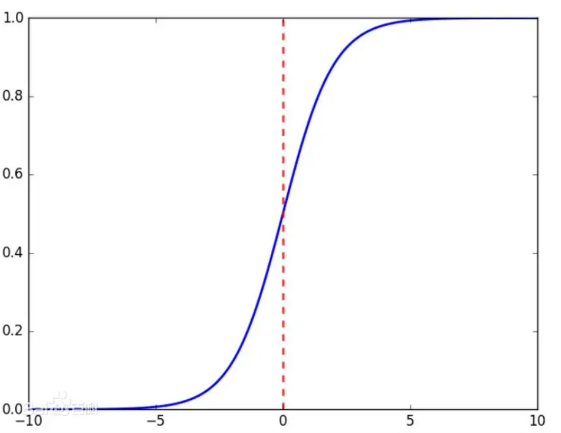
\includegraphics[width=0.4\textwidth]{sigmoid.png}
\end{figure}

公式是$f(x)=\frac{1}{1+e^{-x}}$。该函数导数最大处为0.25,可能导致梯度消失。

Sigmoid函数的导数值可以由函数值来表示成$f'(x)=f(x)\cdot(1-f(x))$

\subsubsection{$Tanh$函数}

Tanh函数是双曲函数中的双曲正切,能将输入映射到$[-1, 1]$之间,图像如图~\ref{fig:tanh}。

\begin{figure}[htb]
	\centering
	\caption{Tanh函数}
	\label{fig:tanh}
	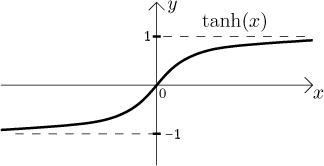
\includegraphics[width=0.4\textwidth]{tanh.png}
\end{figure}

公式是$f(x)=\frac{e^x-e^{-x}}{e^x+e^{-x}}$。该激活函数常用于RNN中。

类似Sigmoid函数,tanh函数的导数值同样可以由函数值表示为$f'(x)=1-f^2(x)$。


\subsection{损失函数}
神经网络的训练过程就是通过梯度下降法最小化损失函数的过程。我们实现了MSE和交叉熵损失函数。

损失函数需要实现$ILossFunction$抽象类中声明的$eval$和
$derive$,它们分别执行求值和求导。如代码~\ref{code:lossfun}。

\begin{lstlisting}[language=c++,style=CppStyle,caption={接口$ILossFunction$},label={code:lossfun}]
class ILossFunction
	: public base::ITypeId
{
 public:
	virtual double operator()(Eigen::VectorXd value, Eigen::VectorXd label) = 0;
	virtual double eval(Eigen::VectorXd value, Eigen::VectorXd label) = 0;
	virtual Eigen::VectorXd derive(Eigen::VectorXd value, Eigen::VectorXd label) = 0;
};
\end{lstlisting}

\subsubsection{MSE损失函数}

MSE是回归损失函数中常用的误差,它是预测值$f(x)$与目标值$y$之间差值平方和的均值。如\eqref{eqn:mse}

\begin{equation}
	\label{eqn:mse}
	MSE(f(x), y) = \frac{1}{n} \sum_{i=1}^n (f(x_i) - y_i)^2
\end{equation}

函数图像如图~\ref{fig:mse}。

\begin{figure}[htb]
	\centering
	\caption{MSE损失函数}
	\label{fig:mse}
	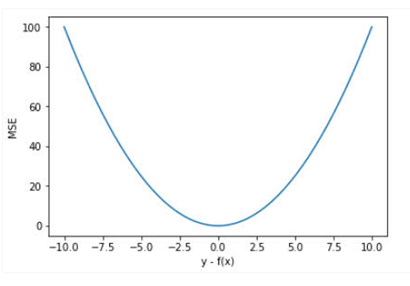
\includegraphics[width=0.4\textwidth]{mse.png}
\end{figure}

平方损失函数是光滑函数,能够用梯度下降方法进行优化,随着误差的减小,梯度也在减小,这有利于收敛,然而预测值和真实值差距越大,
平方损失的惩罚力度越大,即它对于异常点比较敏感,受异常数值影响较大。如果样本中存在离群点,MSE会给离群点更高的权重,
这就会牺牲其他正常点数据的预测效果,最终降低整体的模型性能。

MSE损失函数向最后⼀层的权重传递梯度时,梯度与最后⼀层的激活函数的导数成正⽐,因此,如果起始输出值⽐较⼤,
也即激活函数的导数⽐较⼩,那么整个梯度幅度更新幅度都⽐较⼩,收敛时间很长。若⼀开始输出值⽐较⼩那么更新速度⽐较好,
收敛也快,因此不稳定。且与输出值与真实值的误差成正⽐。

\subsubsection{交叉熵损失函数}

交叉熵损失函数的标准形式如\eqref{eqn:cross-entropy}

\begin{equation}
	\label{eqn:cross-entropy}
	CE(f(x), y) = \frac{1}{n} \sum_{i=1}^n -y_i \log(f(x_i)) - (1-y_i) \log(1-f(x_i))
\end{equation}

其中$x_i$表示样本,$y_i$表示实际的标签,$n$表示样本总数量。它本质上也是一种对数似然函数,
可用于二分类和多分类任务中。当使用sigmoid作为激活函数的时候,常用交叉熵损失函数而不用均方误差损失函数,
因为它可以完美解决平方损失函数权重更新过慢的问题,具有“误差大的时候,权重更新快;误差小的时候,权重更新慢”的良好性质。
此时损失函数对于最后⼀层权重的梯度不再跟激活函数的导数相关,只跟输出值和真实值的差值有关,此时收敛较快。
⼜因为反向传播是连乘的,因此整个权重矩阵的更新都会加快。另外,多分类交叉熵损失求导更简单,损失仅与正确类别的概率有关。


\subsection{优化器}

我们实现了简单的梯度下降优化器和有动量优化和Nestrov优化的SGD优化器。

\subsubsection{简单优化器}

简单优化器实现了简单的定步长梯度下降,即公式\eqref{eqn:gradient_descent}。

\begin{equation}
	\label{eqn:gradient_descent}
	w_i^{(t+1)} = w_i^{(t)} - \alpha \frac{dJ}{dw_i}
\end{equation}

这是一种基础的优化器。其中$\alpha$是学习率。它的选择对效果有很大的影响。

\subsubsection{SGD优化器}
我们实现了和pytorch中的SGD功能同样强大的SGD优化器,这包括动量优化和Nestrov优化。

SGD中动量优化的概念使得前几轮的梯度也会加入到当前的计算中(会有一定衰减),
通过对前面一部分梯度的指数加权平均使得梯度下降过程更加平滑,减少动荡,收敛也比普通的SGD快。
当前梯度方向与累计梯度方向一致时,梯度会被加强,从而这一步下降幅度增大,
若方向不一致,则会减弱当前下降的梯度幅度。更新方式如\eqref{algo:sgdmom}

\begin{algorithm}[htbp]
	\caption{动量优化的梯度下降}
	\label{algo:sgdmom}
	\begin{algorithmic}[1]
		\If{$momentum>1$}
		\State $\mathbf{b}_{t} \gets momentum*\mathbf{b}_{t-1}$
		\Else
		\State $\mathbf{b}_{t} \gets grads$
		\EndIf
	\end{algorithmic}
\end{algorithm}	

动量主要解决SGD的两个问题:
\begin{enumerate}
	\item 随机梯度的方法(引入的噪声);
	\item Hessian矩阵病态问题(可以理解为SGD在收敛过程中和正确梯度相比来回摆动比较大的问题)。  可以形象化的理解为,当前权值的改变会受到上一次权值改变的影响时,类似于小球向下滚动的时候带上了惯性。这样可以加快小球向下滚动的速度。
\end{enumerate}
SGD的优势是:
\begin{itemize}
	\item 相较于非随机算法,SGD能更好的利用、排除冗余信息。
	\item SGD在前期的迭代效果卓越。
	\item 在样本数量较大时,SGD的计算复杂度具有优势
	梯度下降在强凸的情况下收敛的速度是线性收敛的,最差情况下,至少需要迭代$O(log(\frac{1}{\epsilon}))$次,才能达到$\left\|\sum_{i=1}^{n} f_{i}\left(x_{t}\right)-f^{\star}\right\| \leqslant \epsilon$的精度,
	加上每次梯度下降计算n个梯度,所以总的计算复杂度是$O(nlog(\frac{1}{\epsilon}))$。
	而SGD,为了达到$\left\|\sum_{i=1}^{n} f_{i}\left(x_{t}\right)-f^{\star}\right\| \leqslant \epsilon$,在最差情况下,我们需要迭代的次数是$O(\frac{1}{\epsilon})$,但是每次就计算一个梯度,所以计算复杂度为$O(\frac{1}{\epsilon})$。
\end{itemize}

Nesterov是对动量方法的一种改进,由Ilya Sutskever提出,它的主要思想是先按照原来的更新方向更新一步,
然后在该位置计算梯度值,然后再用这个梯度值修正最终的更新方向。如\eqref{eqn:nesterov}。
\begin{equation}
	\label{eqn:nesterov}
	\delta x_t=\rho \Delta x_{t-1}-\mu \Delta f(x_t+\rho \Delta x_{t-1})
\end{equation}

我们整体的SGD实现参照pytorch完成,如算法~\ref{algo:sgd}
\begin{algorithm}[htbp]
	\caption{SGD优化器更新算法}
	\label{algo:sgd}
	\begin{algorithmic}[1]
		\Input{$\gamma\mbox{(学习率)},f\mbox{(目标函数)},\lambda\mbox{(权重衰减)},\mu\mbox{(动量)}$}
		\Input{$\tau \mbox{(抑制参数)},nestrov\mbox{(是否使用nesterov优化)}$}
		\Input{$maxmize\mbox{(是最大化还是最小化)}$}
		
		\For{$t=1 \ \mathop{to} \ \ldots $}
		\State $g_t\gets\nabla_\theta f(\theta_{t-1})$
		\If{$\lambda \ne 0$}
		\State $g_t\gets g_t+\lambda \theta_{t-1}$
		\EndIf
		\If{$\mu \ne 0$}
		\If{$t>1$}
		\State $b_t\gets \mu b_t+(1-\tau)g_t$
		\Else
		\State $b_t\gets g_t$
		\EndIf
		\If{$nesterov$}
		\State $g_t\gets g_{t-1}+\mu b_t$
		\Else
		\State $g_t\gets b_t$
		\EndIf
		\EndIf

		\If{$maxmize$}
		\State $\theta_t\gets\theta_{t-1}+\gamma g_t$
		\Else
		\State $\theta_t\gets\theta_{t-1}-\gamma g_t$
		\EndIf
		\EndFor
	\end{algorithmic}
\end{algorithm}	

\subsection{层与正则化}

层是模型构建中的主体,它要实际地处理反向传播的过程。我们在实现了最为关键也最为基础
的全连接层的基础上,也实现了常见的用于进行正则化的层,如LayerNorm和DropOut。

\subsubsection{全连接层}

全连接层是一种基础的层,它用于建模最基础的含有$n$个神经元的层。
前向传播公式为\eqref{code:forward},
\begin{equation}
	\label{eqn:forward}
	z^l=f(\boldsymbol{W}^l\boldsymbol{x}+\boldsymbol{b}^l)
\end{equation}
反向传播公式如\eqref{eqn:fc_backprop}。
\begin{equation}
	\label{eqn:fc_backprop}
	\boldsymbol{\delta}^l=((\boldsymbol{\omega}^{l+1})^\mathsf{T}\boldsymbol{\delta}^{l+1})\odot f'(\boldsymbol{z}^{l})
\end{equation}

\subsubsection{LayerNorm层}

Layer Normalization\cite{ba2016layer}的作用是减少曾与层之间的协变偏差(Covariate Shift),加快收敛,
在Transformer结构的网络中特别常用。它的前向传播公式如\eqref{eqn:layernorm}。
\begin{equation}
	\label{eqn:layernorm}
	\boldsymbol{z}^l=\boldsymbol{g^l}\odot\frac{1}{\sqrt{\sigma^2+\epsilon}}\left(\boldsymbol{x}-\mu_l\right)+\boldsymbol{b}^l
\end{equation}
其中$\sigma$和$\mu$是输入值标准差和均值,$g_i$和$b_i$是可学习的参数。
反向传播公式如\eqref{eqn:ln_backprop}。

\begin{equation}
	\label{eqn:ln_backprop}
	\begin{aligned}
		&D= (\sigma^2+\epsilon)^{-\frac{1}{2}}\\
		&\frac{\partial J}{\partial x_i}=D\left[\frac{\partial J}{\partial y_i}g_i-\frac{1}{H}\left(\sum_{j=1}^H\frac{\partial J}{\partial y_i}+\hat{x_i}\sum_{j=1}^H\frac{\partial J}{\partial y_j}g_j\cdot \hat{x_j}\right)\right]\\
		&\frac{\partial J}{\partial g_i}=\frac{\partial J}{\partial y_i}\cdot \hat{x_i} \\
		&\frac{\partial J}{\partial b_i}=\frac{\partial J}{\partial y_i}\cdot 1 \\
		&\delta_i=\frac{\partial J}{\partial x_i}
	\end{aligned}
\end{equation}

实验证明,该层对较深的ANN相当有用。

\subsubsection{DropOut层}

DropOut\cite{srivastava2014dropout}在神经网络训练过程中随机选中一些神经元并将其隐藏,然后进行
训练和优化。是一种常见的正则化手段。它的前向传播公式如\eqref{eqn:dropout}。
\begin{equation}
	\label{eqn:dropout}
	\begin{aligned}
		r_j^{(l)} &\sim \mathop{Bernoulli}(p) \\
		\widetilde{\boldsymbol{y}}^{(l)}&=\boldsymbol{r}^{(l)}\odot\boldsymbol{y^{(l)}} \\
	\end{aligned}
\end{equation}
反向传播公式如\eqref{eqn:droupout_backprop}。
\begin{equation}
	\label{eqn:droupout_backprop}
	\frac{\partial J}{\partial \boldsymbol{x}}=\frac{\partial J}{\partial \boldsymbol{y}}\odot \boldsymbol{r}^{(l)}
\end{equation}

\subsection{模型}

模型是我们框架的核心。它要处理训练的具体过程和参数的加载与保存。这是神经网络训练和使用
过程中的核心任务

\subsubsection{训练}

对模型的训练和评估任务,我们提供了$train$和$evaluate$方法。他们的主体部分相似,区别
在于$train$计算完损失函数以后,会进一步开始反向传播过程和参数优化过程,而$evaluate$不会。

在训练过程中,损失函数的数值、各测度,例如Top-k accuracy,对神经网络的训练者而言是重要的
参考。为了能够在输出信息的过程中实现高可扩展性的愿景,我们定义了接口$IModelCallback$,
它包括各个环节中可能会用到的回调函数定义。$train$和$evaluate$方法会在特定的阶段调用它们,
并且提供合适的参数以供使用者计算各种参量。如代码~\ref{code:outputcallback}。
\begin{lstlisting}[language=c++,style=CppStyle,caption={接口$IModelCallback$},label={code:outputcallback}]
class IModelCallback
{
 public:
	template<typename T, typename... Args>
	static inline std::shared_ptr<IModelCallback> make(Args&& ... args)
	{
		return std::make_shared<T>(std::forward<Args>(args)...);
	}

	virtual std::string before_world() = 0;
	virtual std::string after_world() = 0;

	virtual std::string before_train(size_t step) = 0;
	virtual std::string train_step(size_t step,
		const dataloader::DataPair& dp,
		Eigen::VectorXd predicts,
		double loss) = 0;
	virtual std::string after_train(size_t epoch) = 0;

	virtual std::string before_eval(size_t epoch) = 0;
	virtual std::string eval_step(size_t step,
		const dataloader::DataPair& dp,
		Eigen::VectorXd predicts,
		double loss) = 0;
	virtual std::string after_eval(size_t epoch) = 0;
};
\end{lstlisting}
为了提供基本的信息输出功能,我们实现了$LossOutputCallback$和
$AccuracyMetricCallback$。它们能够输出损失函数值
和Top-k accuracy测度。

\subsubsection{加载和保存}

为了实现模型的加载与保存,我们要求层的实现提供$Load$和$Save$方法。
在需要保存和加载时,模型会依次对各层调用相应的方法,来将参数写入
流中,或从流中读取。C++的输入输出流是恰当地管理数据输入输出的统一接口,
它是十分强大而有效的。

\subsection{数据和数据加载}

数据是神经网路训练中不可缺少的部分。我们将数据的加载和使用分为$IDataset$和
$Dataloader$两个类来完成。$IDataset$提供了一组实现读取数据集所必需的
接口。为适配任何一种数据集,只要继承该类就能使这个数据集和我们的框架配合使用。

$Dataloader$提供了将数据给到模型进行训练的过程中不可缺少的重要功能,例如按
一定大小取Batch、随机打乱测试数据等,为模型类提供了一个统一的接口。

\section{代码编写}

在代码编写中,我们秉承可靠、安全、现代的理念,积极使用语言新特性、严格按照
编码规范,使得项目有较高的代码质量、更加适应现代C++的演进方向,富有前瞻性。

\subsection{Concept的使用}

在C++20标准诞生之前,为了更有效地利用模板,人们使用SFINAE(Substitution Failure Is Not An Error)
来对模板的类型参数加以限制。这种方法很不直观、实现复杂、会导致编译器输出长度较高、内容混杂、
甚至无法被理解的错误信息。是一种具有时代局限性的做法。

然而不对模板参数加以限制,就会导致错误在编译期模板实例化时报错,错误信息也难以被理解,
并且不方便IDE和静态分析工具对程序进行分析。

因此,我们使用了C++20引入的Concept特性对模板参数加以限制。类模板、函数模板和类模板的成员都可以
和一个约束相关联,它指定了对模板参数的要求,可以被用于选择最正确的函数重载和模板的特化。而有名称的
一个要求的集合称之为\emph{Concept}。每一个Concept都是一个谓词,它在编译期被计算。

例如我们定义了如代码~\ref{code:concept}中的Concept。
\begin{lstlisting}[language=c++,style=CppStyle,caption={Concept},label={code:concept}]
template<typename T>
concept IterableData=
requires(T t)
{
    { t.begin() };
    { t.end() };
};

template<typename T>
concept SizedData=
requires(T t, int i)
{
    { t.size() }->std::convertible_to<size_t>;
    { t.get(i) };
};
\end{lstlisting}
这段代码被用于模型类的实现中。它们分别约束要求提供STL式的迭代器接口和Python-like的容器大小/获取项目接口。
由于Concept现在会参与重载决议,因此有如代码~\ref{code:concept_usage}中的重载函数就可以按照数据集对象提供的具体接口而选择
正确的重载版本来完成预测工作。这大大地提高了接口的泛用性,既使用了统一的接口,又为数据集实现提供了更大的自由。

\begin{lstlisting}[language=c++,style=CppStyle,caption={Concept的使用},label={code:concept_usage}]
template<IterableData T>
std::vector<base::VectorType> predict(const T &dataset)
{
	std::vector<base::VectorType> ret{};
	for (const auto &d: dataset)
	{
		const auto &[data, label] = d;
		ret.push_back((*this)(data));
	}
	return ret;
}
template<SizedData T>
std::vector<base::VectorType> predict(const T &dataset)
{
	std::vector<base::VectorType> ret{};
	for (int i = 0; i < dataset.size(); i++)
	{
		auto [data, label] = dataset.get(i);
		ret.push_back((*this)(data));
	}
	return ret;
}
\end{lstlisting}

\subsection{编码规范}

为了提高代码质量,保证可维护性,我们严格执行了编码规范。在代码风格上,我们
按照\textit{谷歌开源项目风格指南}\cite{weinberger2013google}的规范进行编写。
有效地保证了代码风格的统一,进而方便错误排查,增强了代码的安全性,同时,也与面向
开源社区的开发方式的要求相适应。同时,该指南对类是否可复制、可移动的要求有效地保证了性能。

在语言功能的取舍上,我们按照\textit{C++ Core Guidelines}\cite{stroustrup2018c++}的指南,
这包括
\begin{itemize}
	\item 使用Concept而不是SFINAE来约束模板
	\item 使用智能指针管理对象的生命周期
	\item 使用GSL
	\item 其他参考该指南的内容
\end{itemize}
这些规则使得编码过程中使用到的功能更符合C++演进的方向,使得代码实现更加安全,
有更少的潜在错误。

\subsection{团队协作}
\begin{figure}[htbp]
	\centering
	\caption{基于Git的团队合作}
	\label{fig:coorp}
	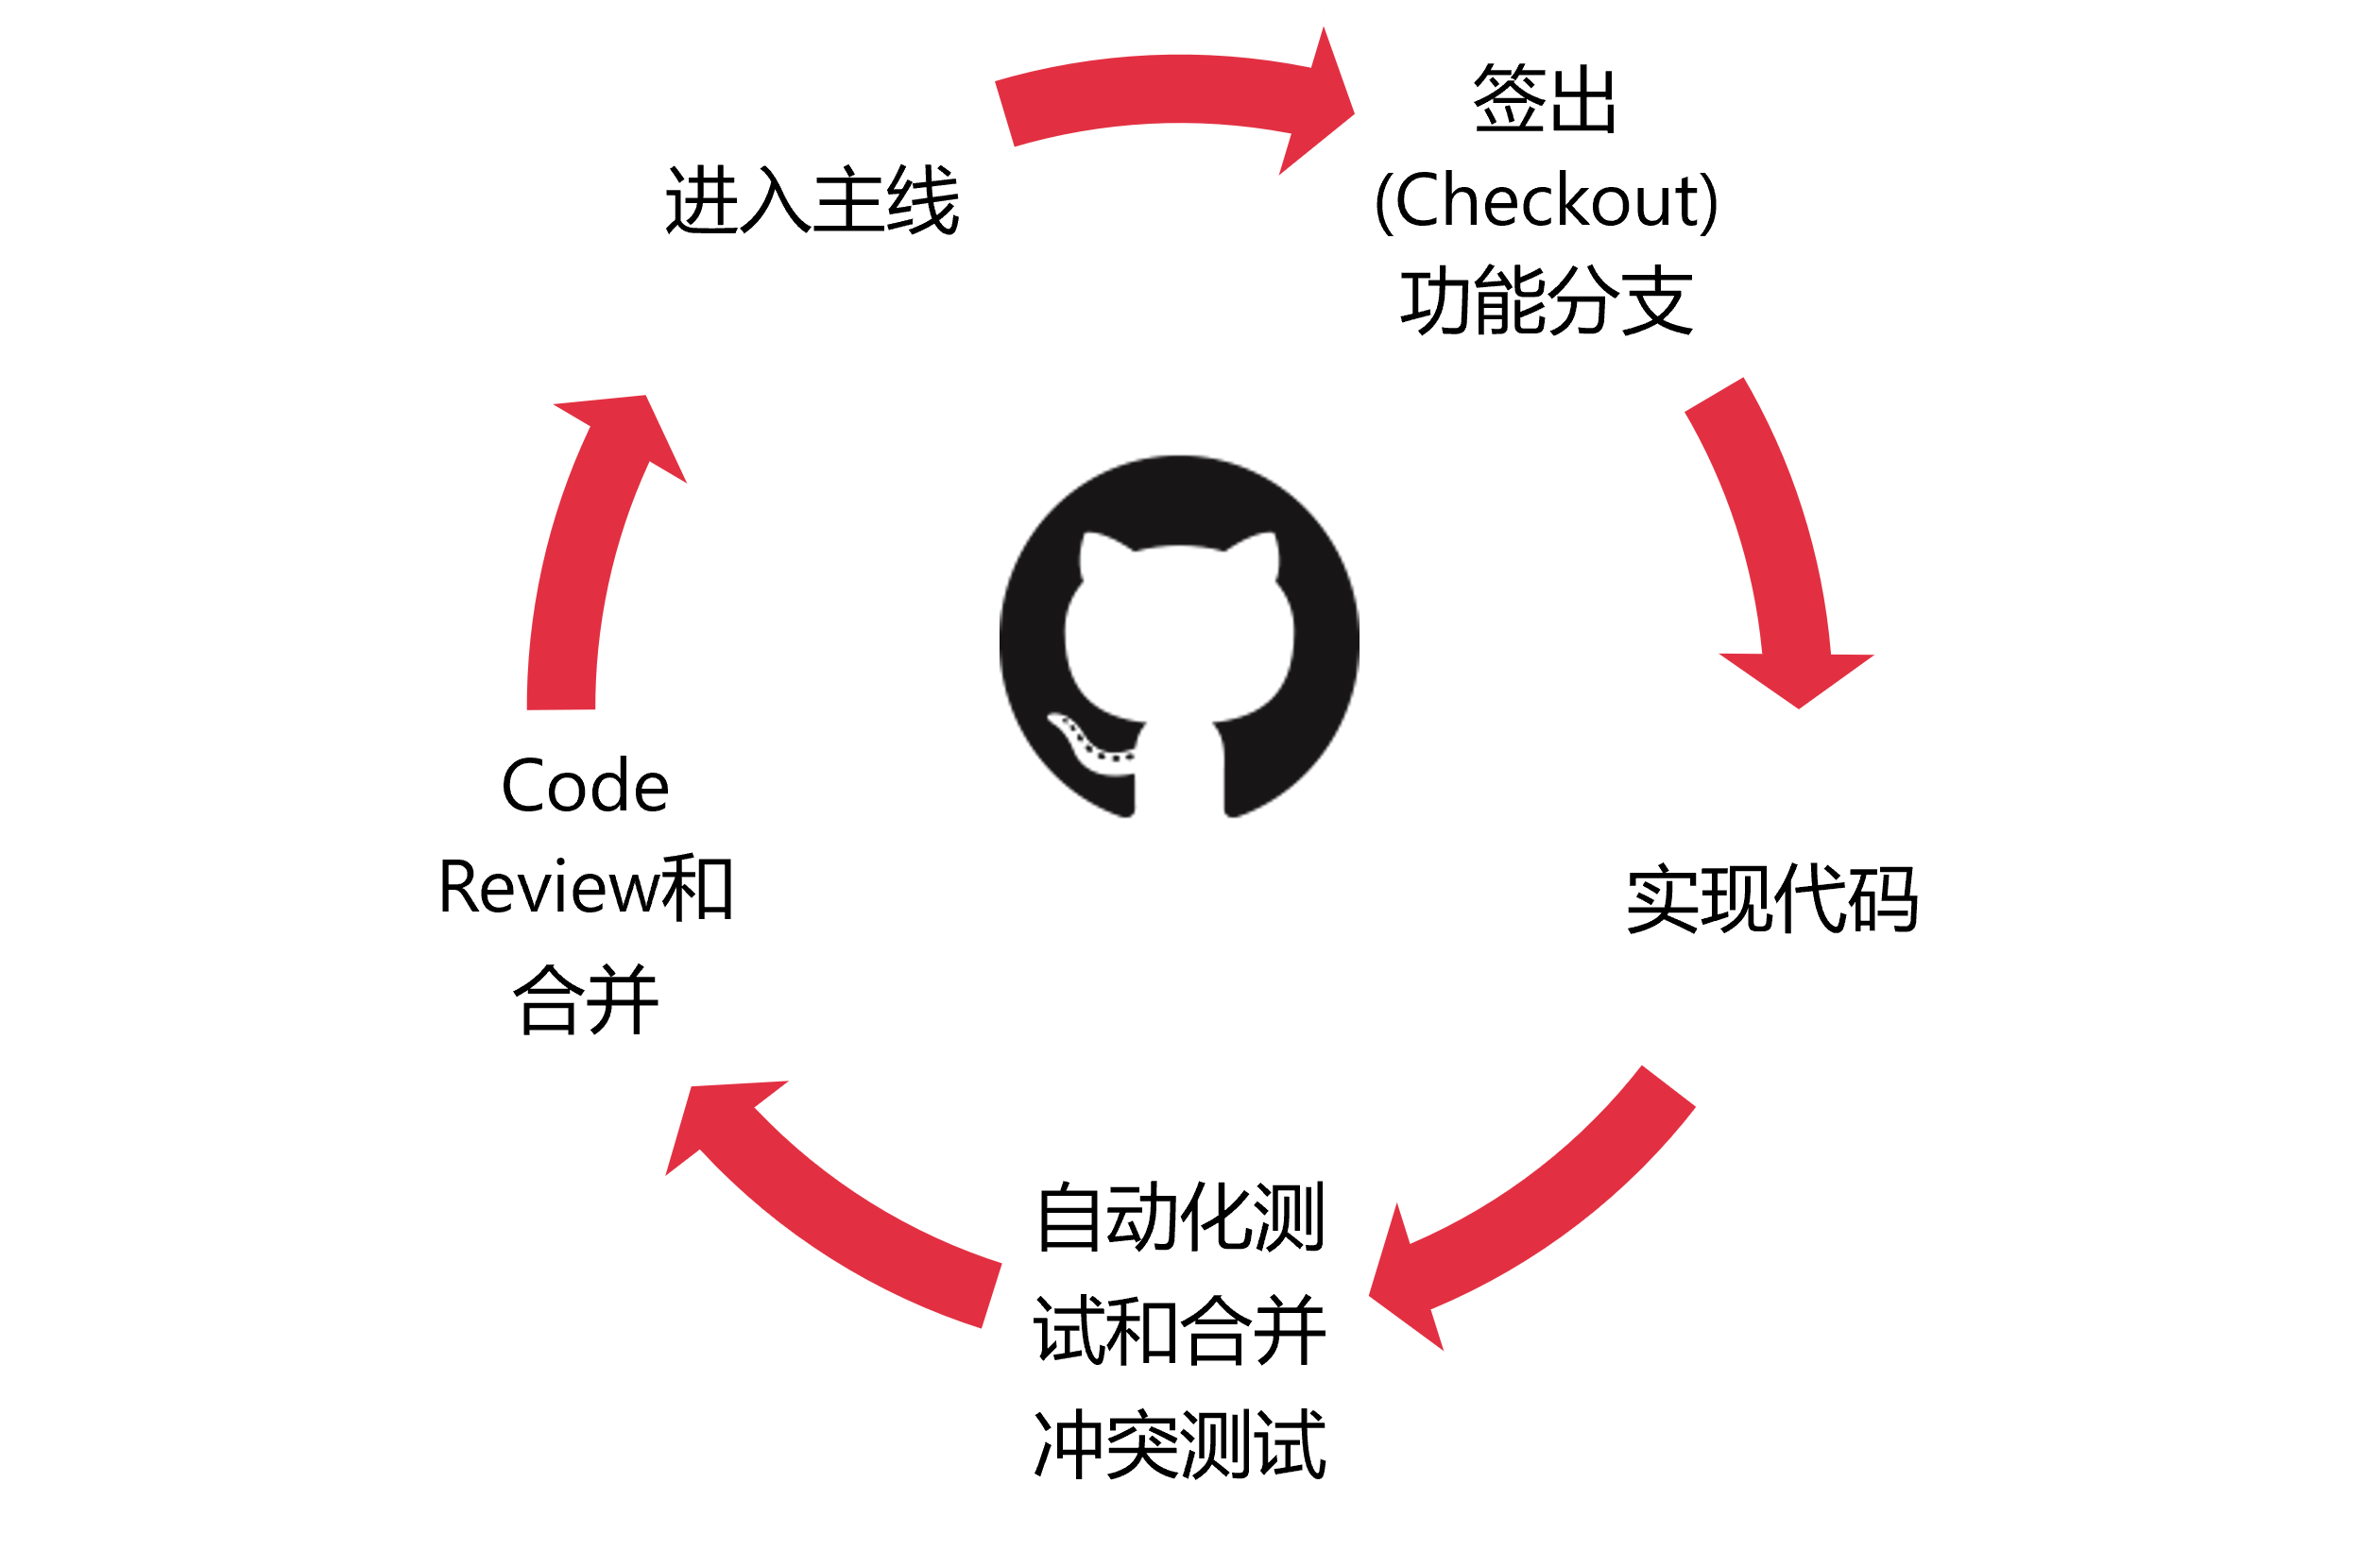
\includegraphics[width=0.4\textwidth]{coorp.png}
\end{figure}
在团队协作上,我们使用了如图~\ref{fig:coorp}所示的基于Git的工作方式。这种方式
在现代软件生产中有很广泛的应用。利用源代码版本控制工具,这种方式实现了修改可溯源
可回滚、合并过程清晰,能够有效结合Github Action进行自动化测试。这既能使开发过程
更为顺利,也能避免人为错误对开发进度和软件质量造成负面影响。

为了进一步确保软件质量,我们基于Google Test为各模块编写了单元测试。单元测试是一种
常用的黑盒测试,是现代软件生产中保证软件质量的重要方式。
\begin{figure}[htbp]
	\centering
	\caption{单元测试}
	\label{fig:unittest}
	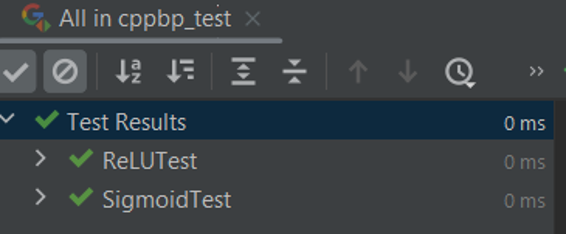
\includegraphics[width=0.4\textwidth]{unitest.png}
\end{figure}

\subsection{数据统计}

使用有名的开源代码量统计工具cloc,我们对项目的代码量进行统计,如表\ref{tbl:code}。

\begin{table}[htb]
	\centering
	\caption{代码量统计}
	\label{tbl:code}
	\begin{tabular}{c|c|c|c|c}
		\toprule
		\hline 
		语言 & 文件 & 空行 & 注释 & 代码 \\
		\hline 
		C++ & 25 & 394 & 83 & 1482 \\
		C++ 头文件 & 38 & 342 & 125 & 868 \\
		Markdown & 1 & 32 & 0 & 79 \\
		CMake & 9 & 34 & 0 & 67 \\
		Yaml & 1 & 0 & 1 & 65 \\
		\hline 
		总计 & 74 & 802 & 209 & 2561 \\
		\hline 
		\bottomrule
	\end{tabular}
\end{table}


\section{实验}

\begin{figure*}[htb]
	\centering
	\subfloat[Iris分类网络结构\label{fig:netiris}]{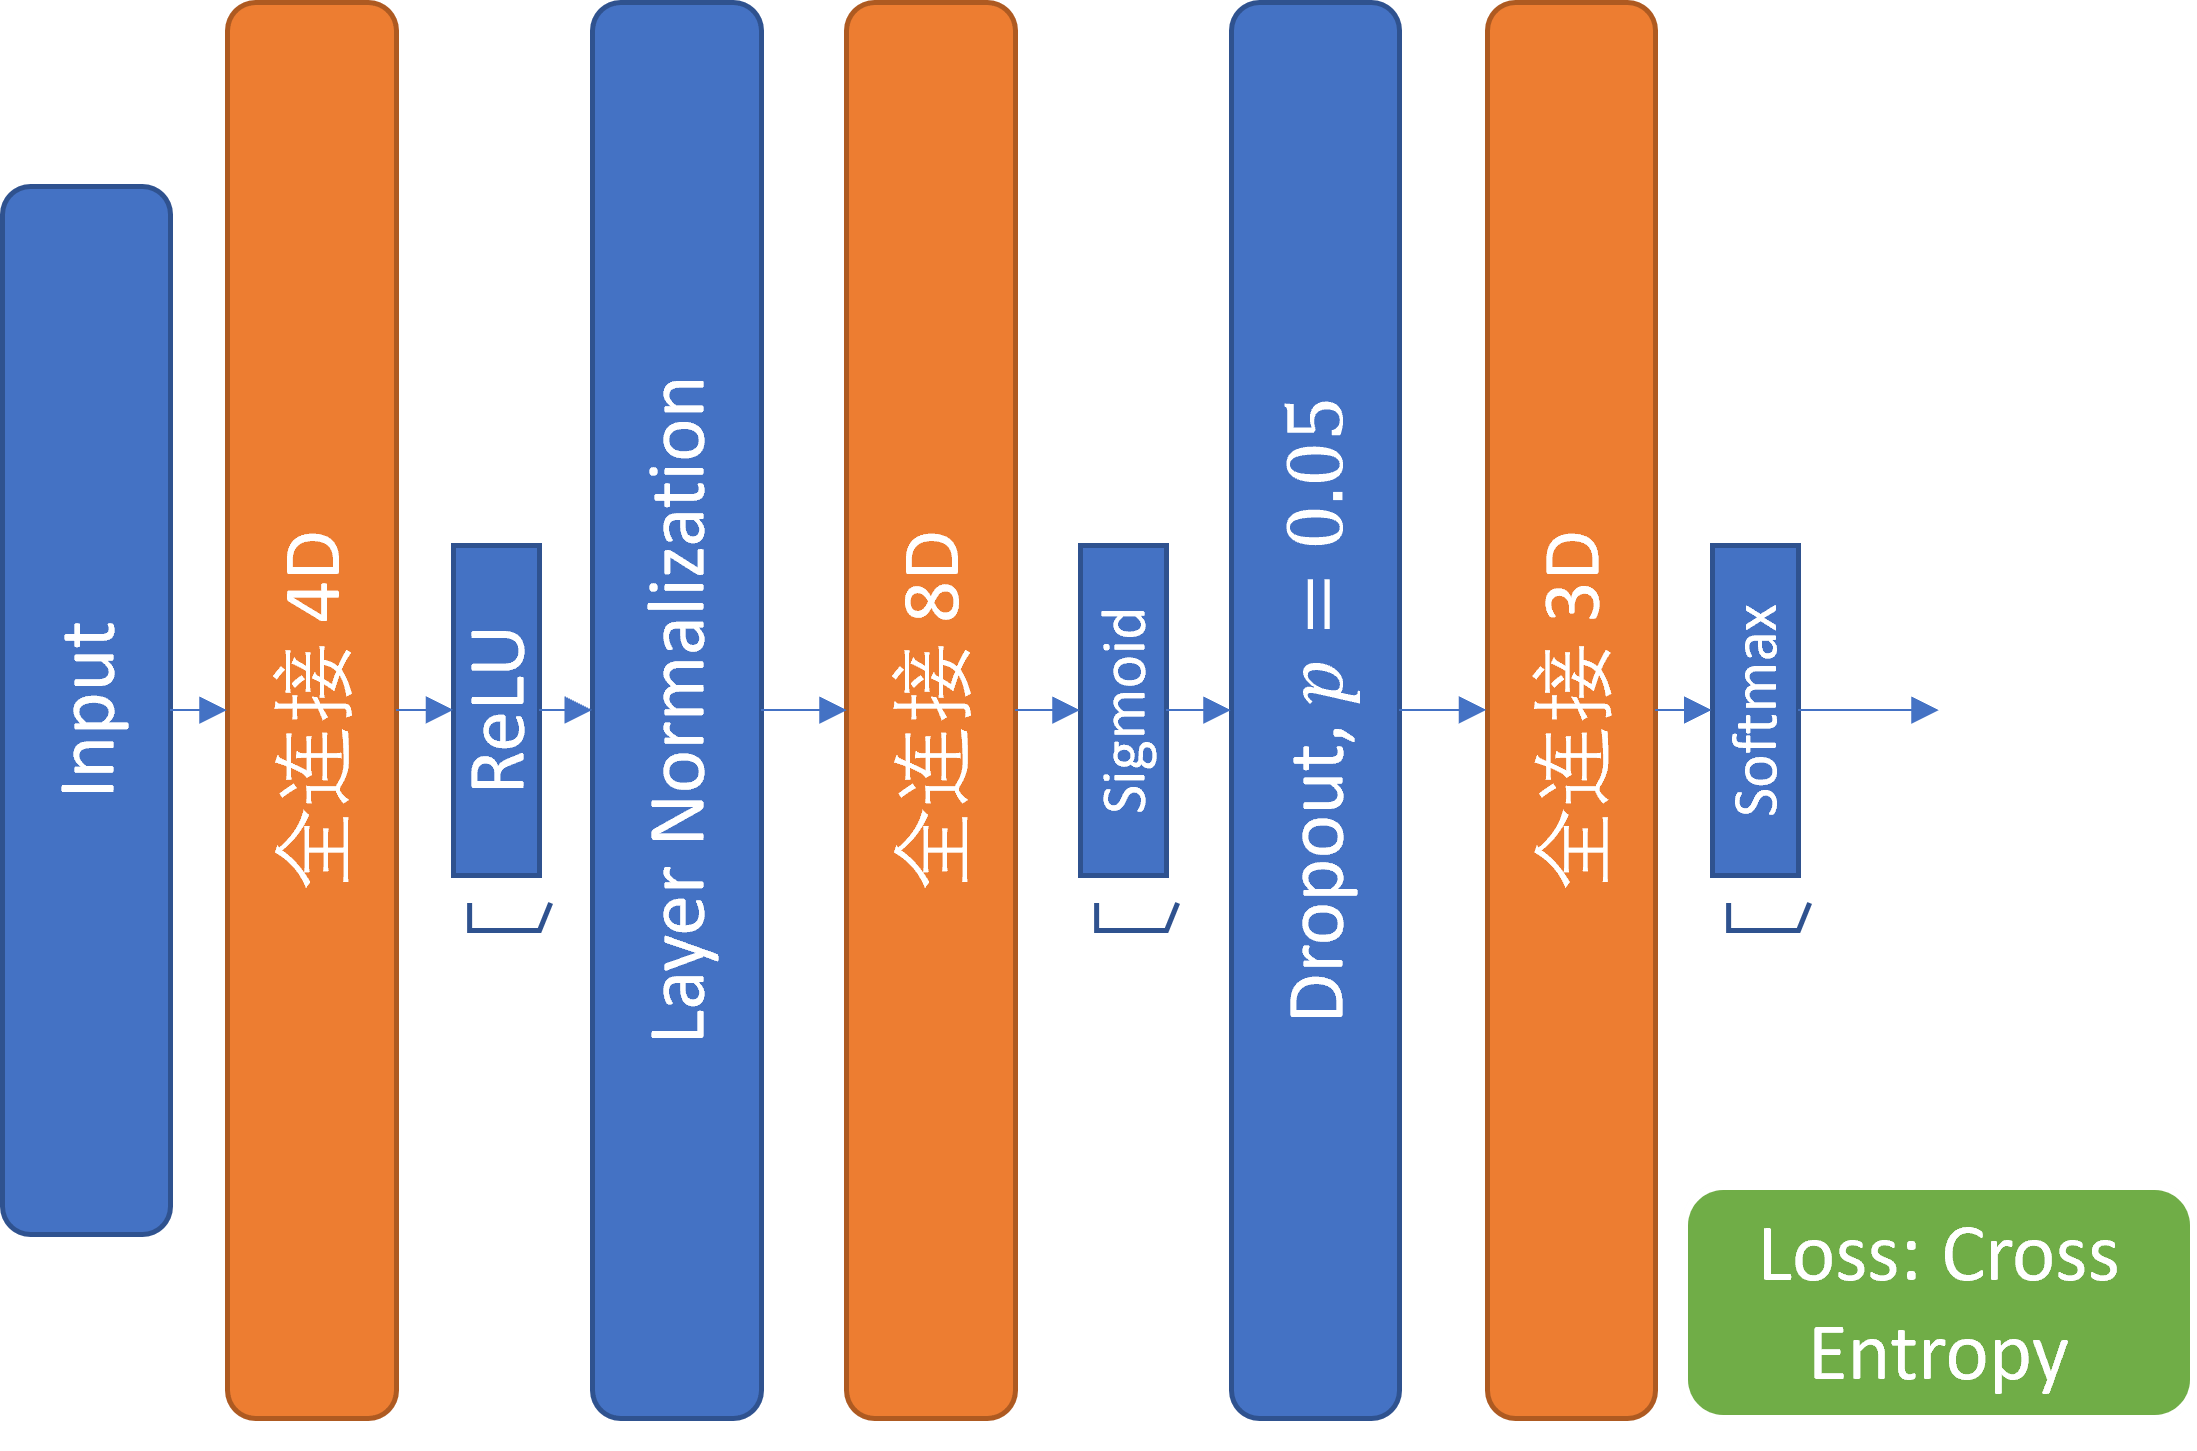
\includegraphics[width=2in]{iris_model.png}}
	\hspace*{1cm} 
	\subfloat[MNIST识别网络结构\label{fig:netmnist}]{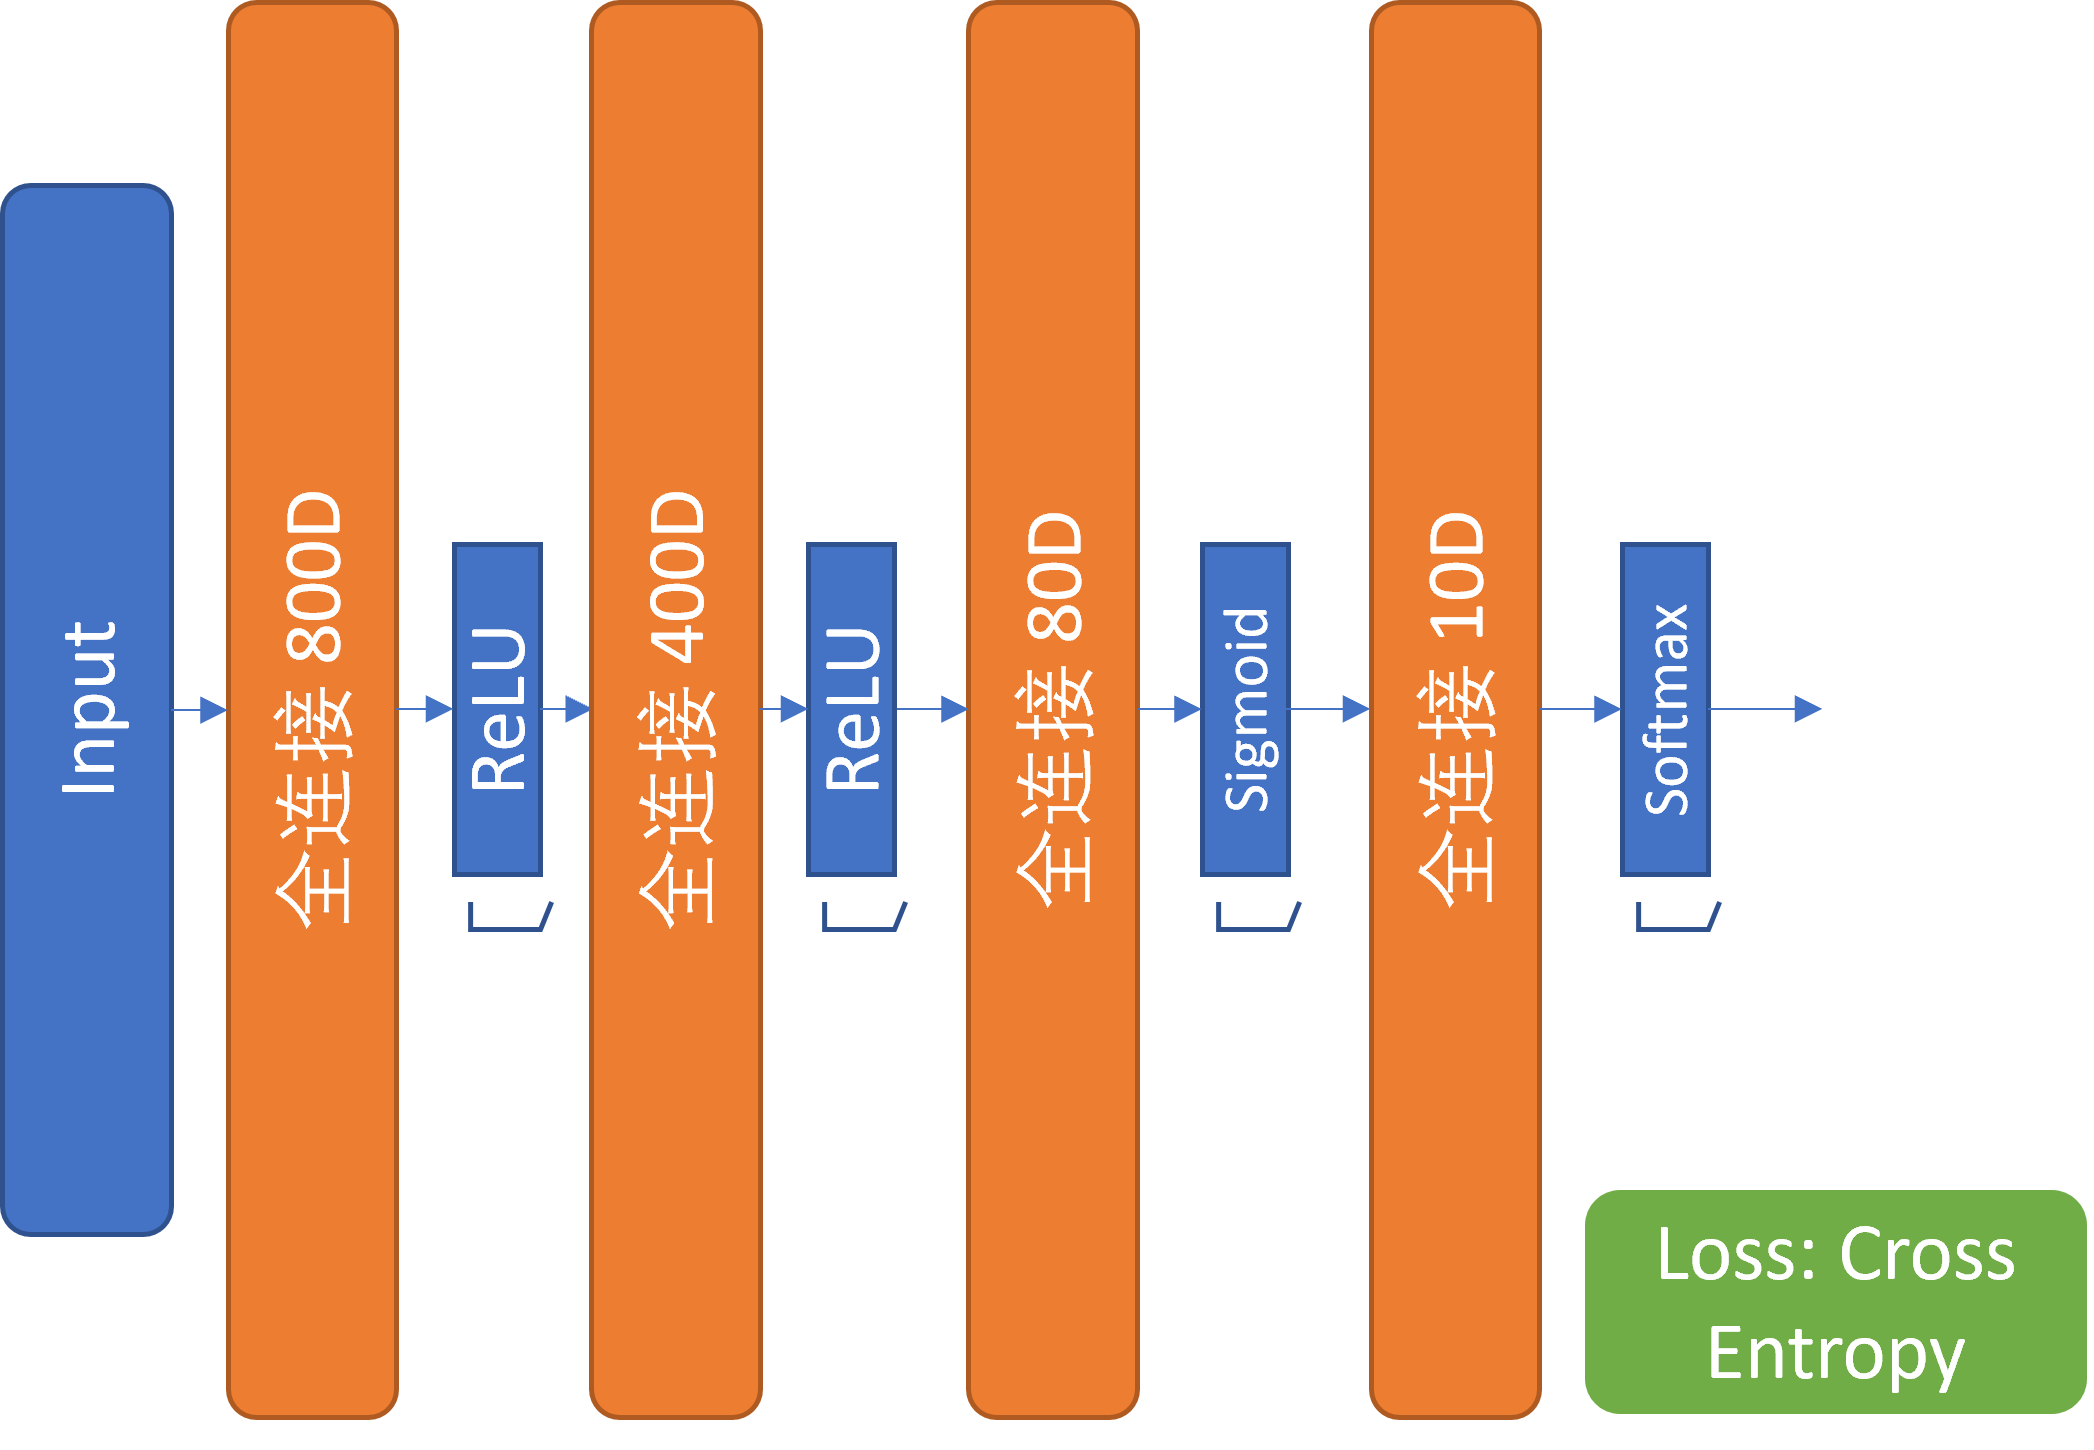
\includegraphics[width=2in]{mnist_model.png}}
	\caption{实验网络结构}
	\label{fig:networks}
\end{figure*}

我们在MNIST数据集和Iris数据集上进行了实验,分别进行鸢尾花分类任务和MNIST图像分类任务。


\subsection{Iris数据集}

Iris数据集是一个较小的常用数据集。它包含了三种鸢尾花的四类不同参数。数据分布见\nameref{sec:iris}
中的图~\ref{fig:iris}。可见该数据集包含了难以线性分类的特征,是测试简单神经网络
的理想数据集。

我们采用了如图~\ref{fig:netiris}的网络结构来完成分类。它使用层规范化层(Layer Normalization)和Drop DropOut层和LayerNorm层
来进行正则化。

在分类任务中,我们使用$8:2$的比例划分训练集和测试集并进行随机打乱。训练方法如表~\ref{tbl:train_iris}。
\begin{table}[htb]
	\centering
	\caption{训练参数}
	\label{tbl:train_iris}
	\begin{tabular}{c|c}
		\toprule
		\hline
		参数 & 值 \\
		\hline
		Batch Size & 16 \\
		学习率 & 0.05 \\
		Epoch & 1000 \\
		损失函数 & Cross Entropy \\
		初始化方法 & Xavier \\
		\hline
		\bottomrule
	\end{tabular}
\end{table}
进行训练之后多次测量,达到了最高99.3\% Top-1 Accuracy和100\% Top-3 Accuracy的准确率。如图~\ref{fig:iris_right}所示。
\begin{figure}[H]
	\centering
	\caption{Iris数据集实验结果}
	\label{fig:iris_right}
	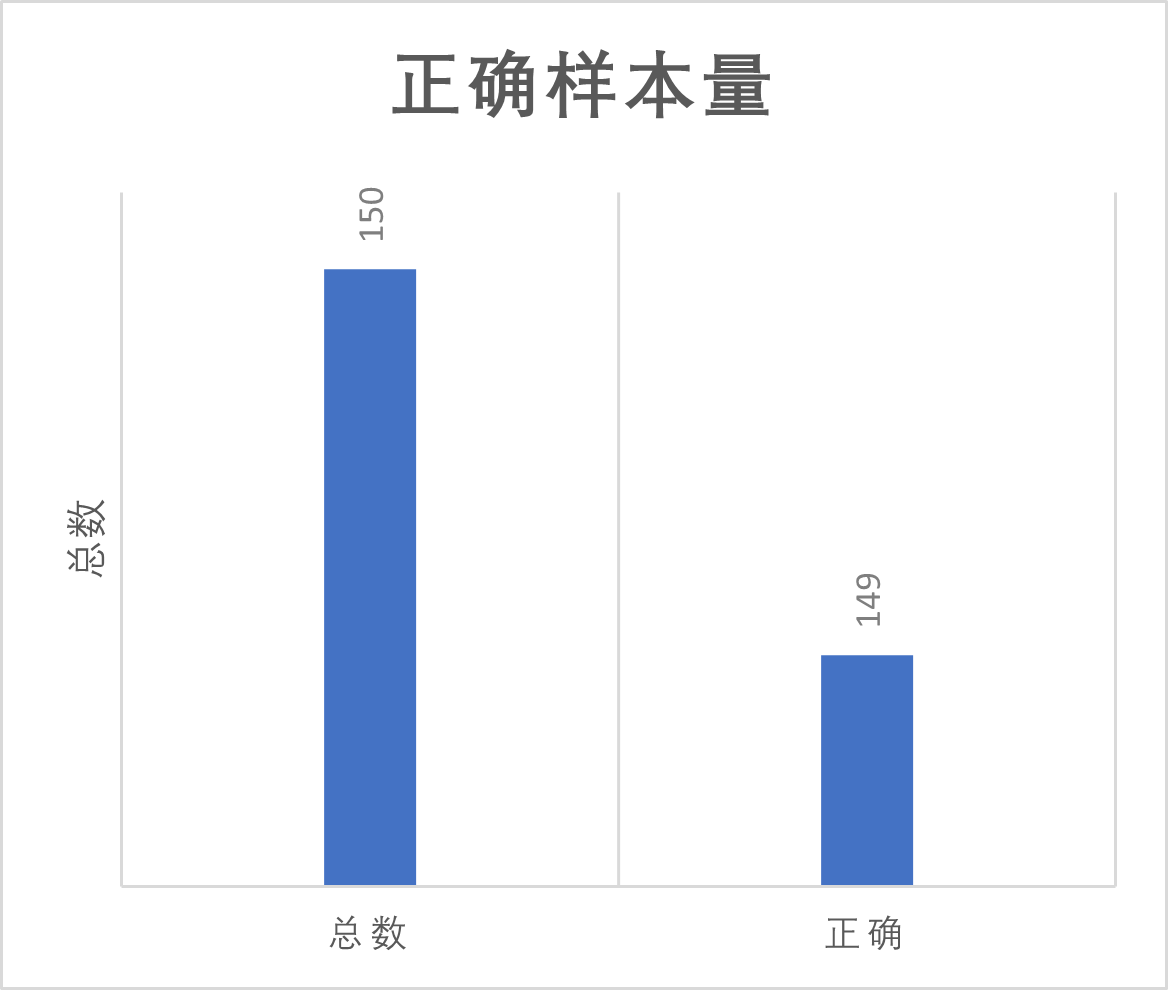
\includegraphics[width=0.4\textwidth]{right_iris.png}
\end{figure}

\subsubsection{消融实验}

为了证明正则化手段的有效性,我们进行了消融实验(Ablation Study),如图~\ref{fig:ablation_iris}(D=Drop Out, LN=Layer Normalization)
\begin{figure}[H]
	\centering
	\caption{消融实验结果}
	\label{fig:ablation_iris}
	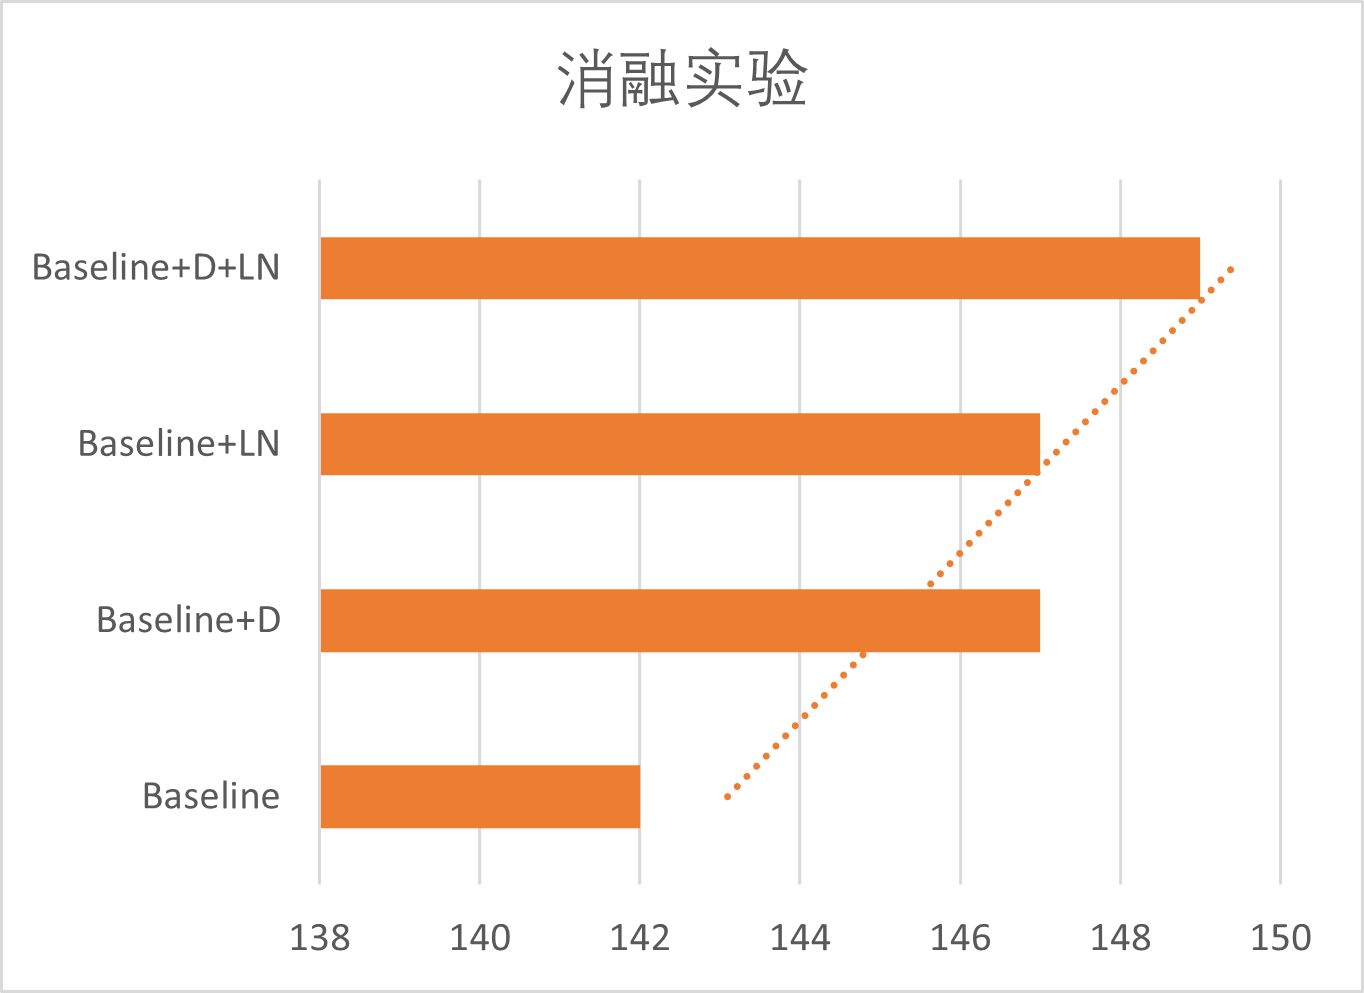
\includegraphics[width=0.48\textwidth]{ablation_iris.png}
\end{figure}

可见Layer Normalization和Drop Out都为提高准确率给出了正贡献。它们的互相作用
没有相互拮抗的现象。


\subsection{MNIST数据集}

Iris数据集是经典的图像分类任务数据集,它由近60000张包含一个手写数字的灰度图组成。
我们使用如图~\ref{fig:netmnist}的网络结构来进行实验。

由于MNIST数据集相对较大。我们没有实现GPU计算,因此训练过程相当缓慢,我们几乎无法
开展进一步的实验。但是在较少轮数的训练之后该简单的全连接神经网络亦达到了80\% Top-1 Accuracy的准确率。
如图~\ref{fig:mnist_result}。

\begin{figure}[H]
	\centering
	\caption{MNIST数据集训练结果}
	\label{fig:mnist_result}
	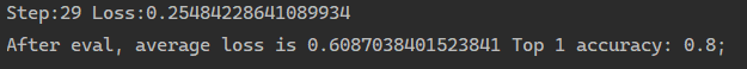
\includegraphics[width=0.4\textwidth]{res_mnist.png}
\end{figure}

\section{结论}

在此次大作业中,我们使用C++完成了一神经网络框架。在这个过程中,我们既体验了现代软件
开发的流程,也使用面向对象的程序设计思想亲自完成了框架的设计和编写。体会到了面向对象
的程序设计思想能够更好地分解和处理问题、更好地组织代码,从而提高程序的可读性和可维护性。
我们实现的神经网络框架在推理速度上达到了与现有成熟框架同一数量级的结果。

\end{spacing}

\clearpage
\onecolumn

\section*{参考文献}
\addcontentsline{toc}{section}{参考文献}

\bibliographystyle{unsrt}
\bibliography{reference}

\appendix
\section*{附录:鸢尾花数据集分布图}
\label{sec:iris}

\begin{figure}[H]
	\centering
	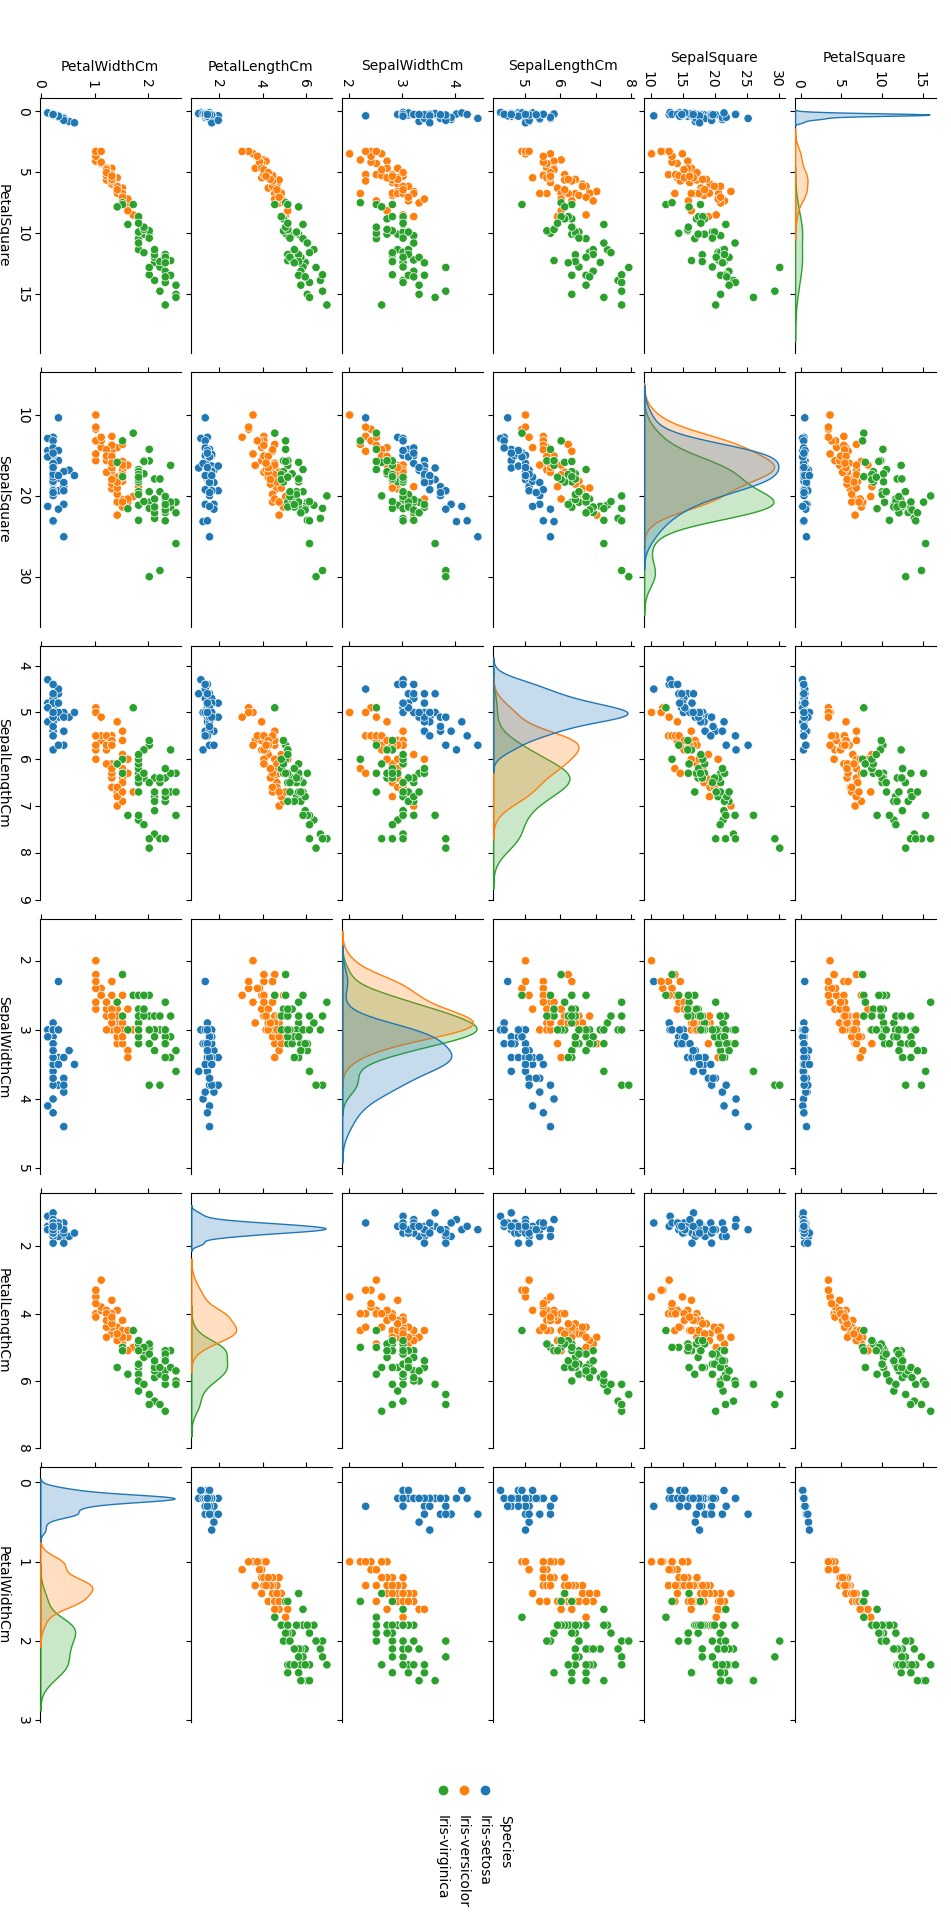
\includegraphics[width=0.7\textwidth]{pairplot.png}
	\caption{Iris数据集数据分布}
	\label{fig:iris}
\end{figure}

\clearpage
\section*{附录:分工}
\addcontentsline{toc}{section}{分工}

\begin{table}[H]
	\centering
	\caption{分工}
	\label{tbl:assignment}
	\renewcommand\arraystretch{1.5}
	\begin{tabular}{c|c}
		\toprule
		\hline
		成员 & 分工 \\
		\hline
		熊恪峥 & \thead{框架整体设计、反向传播的公式推导、变形和实现、框架主体代码编写;\\ 报告撰写和整理、PPT制作、上台汇报。} \\
		\hline
		徐杰 & 反向传播的公式推导、变形;交叉熵损失函数的实现;Softmax激活函数实现;部分报告撰写\\
		\hline
		杨夏婕 & SGD优化器实现;部分报告撰写\\
		\hline
		黄彬茹 & ReLU和Tanh激活函数实现;部分报告撰写\\
		\hline
		\bottomrule
	\end{tabular}
\end{table}


\end{document}